%!TEX root = ../thesis.tex
%*******************************************************************************
%****************************** Second Chapter *********************************
%*******************************************************************************

\chapter{Marco teórico}

\ifpdf
    \graphicspath{{Chapter2/Figs/Raster/}{Chapter2/Figs/PDF/}{Chapter2/Figs/}}
\else
    \graphicspath{{Chapter2/Figs/Vector/}{Chapter2/Figs/}}
\fi


\section{Tecnologías}

\subsection{HTTP}

HTTP, Hypertext Transfer Protocol (Protocolo de Transferencia de Hipertexto) por sus
siglas, es el protocolo por el cual se comunican navegadores, servidores y aplicaciones
relacionadas con la web alrededor de todo el mundo.

Este protocolo se encuentra en la capa de aplicación del modelo OSI. Ha estado en uso por
la World-Wide Web (WWW) desde 1990. Su primera versión hace referencia a HTTP/0.9 y era un 
protocolo simple para la transferencia de datos a través de la internet.

HTTP/1.0 surge a través de la definición del RFC 1945, este mejoró sustancialmente la
comunicación permitiendo a los mensajes encontrarse en formato MIME (Multipurpose
Internet Mail Extensions). Los servidores web adjuntan un tipo MIME a todas sus peticiones
HTTP. Cuando un navegador web obtiene una respuesta desde un servidor, mira el tipo MIME
asociado a ella para ver si sabe cómo manejar el archivo. La mayoría de los navegadores
pueden manejar cientos de tipos de archivos populares: Imágenes, videos, sonidos,
documentos de texto, entre otros.

La última versión de este procolo es la 2.0, definida en el RFC 7540 en el año 2015. Un
gran avance en esta última versión contribuye a disminuir el tráfico innecesario en 
la red definiendo un mapeo optimizado de la semántica de HTTP a una conexión subyacente.

El modo de funcionamiento es muy sencillo. Esta compuesto por dos partes quienes son 
las partes que se comunican, estas son el cliente y el servidor. Básicamente el cliente
envía peticiones al servidor y este debe servirlas en caso de poder. De lo contrario, 
el servidor devolverá el error correspondiente a alguna de las posibles causas. Algunas 
de las más comunes son que el recurso que el servidor busca no se encuentre, que el 
recurso no esté disponible, que se haya movido de lugar o que haya habido algún error 
interno.

\begin{figure}[htbp!] 
\centering    
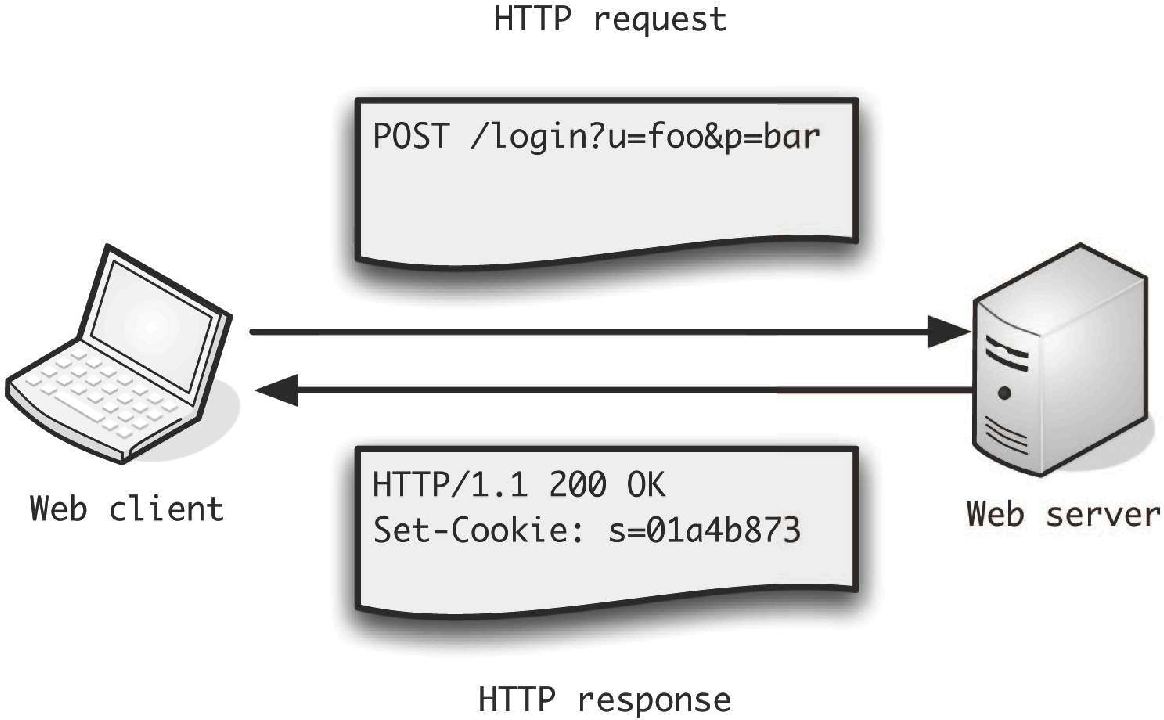
\includegraphics[width=0.5\textwidth]{http1}
\caption[HTTP]{Este es el comportamiento con información básica del protocolo HTTP}
\label{fig:http-behavior}
\end{figure}


\subsection{API REST}

La sigla REST responde a Representational State Transfer- Transferencia de Estado
Representacional. Es cualquier interfaz entre sistemas que use HTTP para obtener
datos o generar operaciones sobre esos datos en todos los formatos posibles, como XML y
JSON. También podemos decir que es un estilo de arquitectura para proveer estándares entre
sistemas de computadoras en la web. 

Su creador, Roy Fielding, es también coautor del protocolo HTTP mencionado en el capítulo 
anterior. REST nace en el año 2000.

La arquitectura REST describe seis restricciones que definen la base del estilo 
RESTful:

\begin{itemize}
   \item first item
   \begin{itemize}
     \item first nested item
     \item second nested item
   \end{itemize}
   \item second item
   \item third item
\end{itemize}


\begin{itemize}
   \item Interfaz Uniforme
	
	Define la interfaz entre clientes y servidores. Simplifica y desacopla la 
	arquitectura. Tiene cuatro principios:
	   
   \begin{itemize}
     \item Basada en Recursos
     
	Los recursos son identificados individualmente en las peticiones usando su URI como
	identificadores. Los recursos en si mismos están separados de lo que terminará siendo 
	su representación devuelta al cliente.     
     
     \item Manipulación de recursos a través de representaciones
     
     Cuando un cliente tiene una representación de algún recurso, esto es suficiente 
     para modificar o eliminar el recurso siempre y cuando se tenga permiso para esto.
     
     \item Mensajes auto descriptivos
     
     Cada mensaje incluye suficiente información describiendo cómo debe éste procesarse.
     
     \item Hypermedia as the Engine of Application State (HATEOAS)
     
     Los clientes entregan el estado a través del contenido del body, los parámetros de
     la query, los headers del request y el URI solicitado (el nombre del recurso). 
     Los servicios entregan estado a los clientes a través del
     body, códigos de respuesta y headers en la respuesta.
   \end{itemize}
   
	\item Sin estado
	
	Esto significa que el estado necesario para manejar la petición está contenido en 
	la petición en si misma como parte de la URI, los parámetros de la query, el body o 
	los headers. La URI identifica de manera única al recurso y el body contiene el estado 
	(o el cambio de éste) de ese recurso. Luego de que el servidor procese lo necesario, 
	la información pertinente es devuelta al cliente mediante headers, estados y el body.
	
	\item Cacheable
	
	Los clientes pueden cachear respuestas. Las respuestas deben definirse a si mismas 
	como cacheables o no cacheables. Esto es para evitar que los clientes reutilicen datos 
	inapropiados u obsoletos.
	
	\item Cliente-Servidor 
	
	La interfaz uniforme separa los clientes de los servidores. Esta separación de 
	conceptos significa que, por ejemplo, los clientes no están envueltos en el guardado 
	de datos, tarea que recae internamente en cada servidor. Por otro lado, los servidores
	no se preocupan por la interfaz de usuario o por el estado de éste. Mientras la 
	interfaz se mantenga, tanto cliente como servidor pueden ser desarrollados y/o 
	reemplazados.
	
	\item Sistema en capas
	
	Un cliente no posee la capacidad por si mismo de decir si está conectado al 
	servidor final o a un servidor intermedio. Los servidores intermedios pueden aumentar 
	la escalabilidad activando balanceadores de carga o caches compartidos.
	
	\item Código en demanda (opcional)
	
	Los servidores son temporalmente capaces de transferir al cliente funcionalidades o 
	código que éstos puedan ejecutar.

\end{itemize}

 
\subsection{AJAX}

\subsection{JWT}

\subsection{Memoria Cache}


\section{Herramientas y tecnologías utilizadas}

\subsection{PHP}

\subsection{Lumen Framework}

\subsection{SQL}

\subsection{Taiga}

\subsection{Vagrant}

\subsection{Git}